\documentclass[tikz,border=10pt]{standalone}
\usetikzlibrary{calc}
\begin{document}
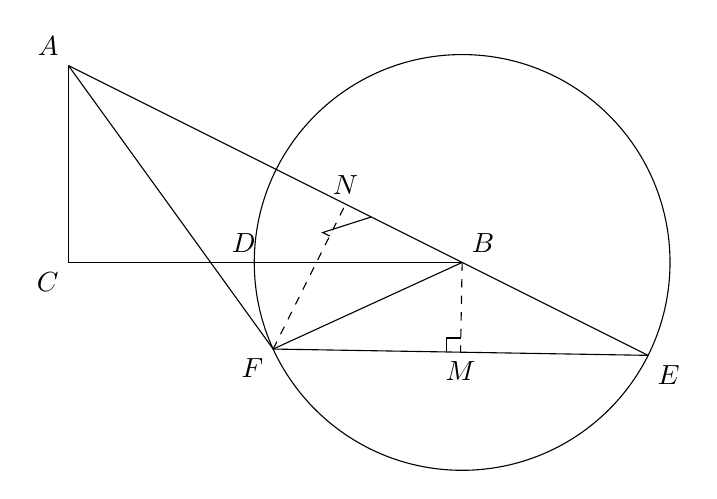
\begin{tikzpicture}[scale=1]
  \coordinate (A) at (0,4);
  \coordinate (C) at (0,1.5);
  \coordinate (D) at (2.5,1.5);
  \coordinate (B) at (5,1.5);
  \coordinate (E) at (7.36,0.32);
  \coordinate (F) at (2.6,0.4);
  \coordinate (M) at (4.98,0.36);
  \coordinate (N) at (3.52,2.24);

  \draw (A) -- (C) -- (B);
  \draw (A) -- (E);
  \draw (A) -- (F) -- (B);
  \draw (F) -- (E);
  \draw[dashed] (F) -- (N);
  \draw[dashed] (B) -- (M);
  \draw (B) circle (2.64);

  % right angle at M
  \draw ($(M)+(-0.18,0)$) -- ($(M)+(-0.18,0.18)$) -- ($(M)+(0,0.18)$);
  % right angle at N
  \draw ($(N)!0.22!(F)$) -- ($($(N)!0.22!(F)$)!0.22!90:(N)$) -- ($(N)!0.22!(B)$);

  \node[above left] at (A) {$A$};
  \node[below left] at (C) {$C$};
  \node[above left] at (D) {$D$};
  \node[above right] at (B) {$B$};
  \node[above] at (N) {$N$};
  \node[below left] at (F) {$F$};
  \node[below] at (M) {$M$};
  \node[below right] at (E) {$E$};
\end{tikzpicture}
\end{document}
